\subsection{On-line K-means}

\mode<presentation>{
\begin{frame} 
    \begin{center} \huge
        \subsecname
    \end{center}
    \begin{center}
		Only use single data point at every iteration.
    \end{center}
\end{frame}
}

\begin{frame}{\subsecname}

\notesonly{We now look at a variant of K-means that partitions the data in an \emph{online} fashion. 
%This allows the clustering to:
}

\begin{figure}[!th]
\footnotesize
\removelatexerror
\begin{algorithm}[H]
  \DontPrintSemicolon
   random initialization of prototypes, e.g.\ $\vec{w}_{q} = \langle  \vec{x} \rangle +\vec{\eta}_{q},\hspace{0.2cm} \vec{\eta}_{q}  \text{ small random vector}$\;
  select learning step:   $0 < \varepsilon  \ll 1$\;
  \Begin(loop){
    choose a data point $\vec{x}^{(\alpha)}$ \;
    assign data point to its closest prototype $q$\;
    \[ q = \argmin_{\gamma} \big| \vec{x}^{(\alpha)} - \vec{w}_{\gamma} \big| \]
    change corresponding prototype according to\;
    \[ \Delta \vec{w}_q = \varepsilon \big( \vec{x}^{(\alpha)} - \vec{w}_{q} \big) \]
    change $\varepsilon$ \;
  }
  \label{alg:on-line-k-means}
  \caption{On-line K-Means}
\end{algorithm}
\end{figure}

\end{frame}
% --------------------------------------------------------------------------

% --------------------------------------------------------------------------
\begin{frame}
\frametitle{Differences between batch and online K-means:}

Online K-means...
\begin{enumerate}
\item adapts to non-stationary data (streaming data)
\slidesonly{
\item less memory
\item faster
\begin{itemize}
    \item Step 1 updates assignment for a single point instead of all 
    \item Step 2 no longer iterates through all points
\end{itemize}
}
\notesonly{
\item mitigates the memory footprint of the algorithm by avoiding having to keep the entire dataset in memory
\item mitigates the time complexity of the algorithm in that  
    \begin{itemize}
    \item we no longer have to update the assignments of all data points (step 1) and that 
    \item updating the prototypes no longer requires iterating through all points (step 2).
    \end{itemize}
    }
\slidesonly{
\item ``Noisiness'' of online K-means allows it to escape local minima.

}
 \notesonly{
\item Online K-means is more robust than batch-learning w.r.t convergence to local minima:
\begin{itemize} 
\item The noisy nature of online K-means gives it a better chance at ``escaping'' local minima. 
\item In batch K-means, $E^T$ either decreases or remains unchanged. Therefore, batch K-means from a local minimum.
\end{itemize}
}
\notesonly{
\item The quality of the solution found by online K-means depends on choosing an appropriate schedule for $\varepsilon$: Robbins-Munro conditions
}
\slidesonly{
\item Choose learning rate schedule for $\varepsilon$: Robbins-Munro conditions
}
\notesonly{(c.f. Fig \ref{fig:annealingScheduleKMeans2})}
\begin{figure}[h!]
  \centering
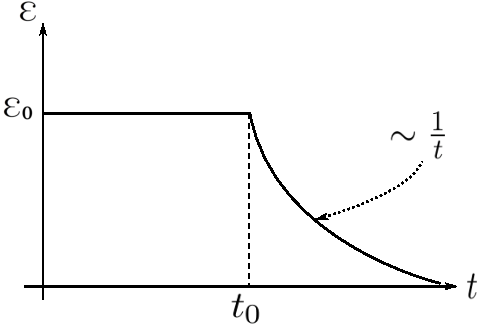
\includegraphics[height=3cm]{img/section4_fig4} 
  \notesonly{\caption{Decaying learning rate schedule to satisfy Robbins-Munro conditions.}}
  \label{fig:annealingScheduleKMeans2}
\end{figure}
\end{enumerate}

A compromise\slidesonly{:}\notesonly{ between batch and online K-means is }\emph{mini-batch K-means}.
\notesonly{One would modify online K-means to operate on a small subset/mini-batch of the data at a time.
}

\end{frame}

\begin{frame}{A local minimum of clustering}

\begin{center}
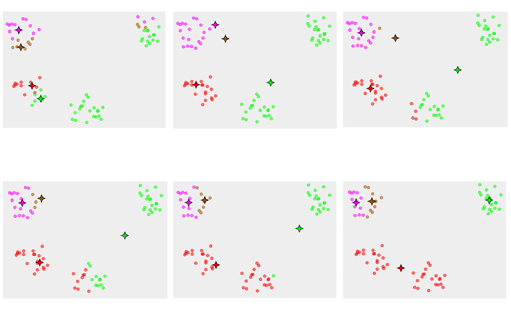
\includegraphics[width=0.7\textwidth]{img/K-means_convergence_to_a_local_minimum_2rows}
\notesonly{\captionof{figure}Example of K-means finding a solution that is a local minimum. Each plot is a snapshot of the prototypes at some iteration of the algorithm.}
\end{center}

\end{frame}

